%% V1.0
%% by Pritesh Gudge, priteshgudge@yahoo.com
%% This is the submission for Inference Project for RoboND

%% Be Udacious!

\documentclass[10pt,journal,compsoc]{IEEEtran}

\usepackage[pdftex]{graphicx}    
\usepackage{cite}
\hyphenation{op-tical net-works semi-conduc-tor}


\begin{document}

\title{Robotic Inference using NVIDIA Digits}

\author{Pritesh Gudge}

\markboth{Inference project, Robotics Nanodegree, Udacity}%
{}
\IEEEtitleabstractindextext{%

\begin{abstract}
The Inference project is a part of the Robotics Nanodegree. The objective was to understand and implement a prototype of vision system for a robotics application.
Two implementations are provided for evaluation. First, the provided dataset of bottles, boxes and other images is used to train a Google Lenet\cite{DBLP} based network and the results are used to classify relevant images provided in the test suite. An average run time for evaluation is approximately 5 milliseconds and the model accuracy of the model is 75.40\% for the given test set. Second, data collection, data conditioning and Google Lenet based model training is used to train a network for food classification.

\end{abstract}

% Note that keywords are not normally used for peerreview papers.
\begin{IEEEkeywords}
Robot, Inference, IEEEtran, Udacity, Deep Learning.
\end{IEEEkeywords}}


\maketitle
\IEEEdisplaynontitleabstractindextext
\IEEEpeerreviewmaketitle
\section{Introduction}
\label{sec:introduction}

\IEEEPARstart{T}{he} progress in the field of robotics is accelarating every day. Robots are being used in many applications like manufacturing, search and rescue, exploration etc. Many of the applications require identifying and detecting objects in multiple scenes and backgrounds. Deep learning is being leveraged into robotic vision and inference as it provides a framework for robots to be configured to operate in multiple environments both natural and man-made. Convolutional and reinforcement learning based techniques have been most effective in robotics applications. Previous approaches to robotic inference were based line follower and other approaches for structured operating environments \cite{linefollower}. Deep learning based approaches provide the possibility to provide identification and detection for robotic inference, given that adequate data is available for training the neural networks. 

In the first part, the provided images of boxes and bottles are used to train an Google Lenet based network for classification. In the second part, a model is trained to classify between fruits and other foods. One can build a diet-tracking or junk food alert robotic system using such a classification model, possibly built into a refrigerator. It generates an alert if unhealthy food is taken out or stored in the refrigerator. A similar model can be used in a robot which sorts items purchased while grocery shopping. Eg. Bananas should not put into the refrigerator, while other fruits can be.
%
%%example for inserting image
%\begin{figure}[thpb]
%      \centering
%      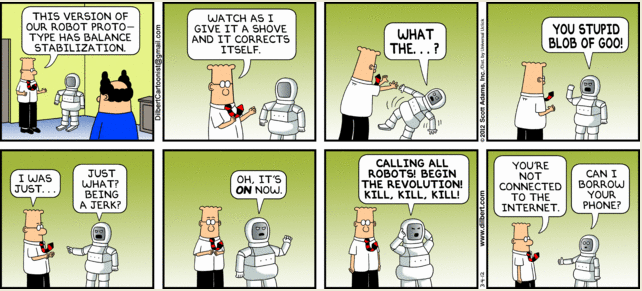
\includegraphics[width=\linewidth]{RobotRevolution5}
%      \caption{Robot Revolution.}
%      \label{fig:robot1}
%\end{figure}
%
%\subsection{Subsection Heading Here}
%Subsection text here.
%
%\subsubsection{Subsubsection Heading Here}
%Subsubsection text here.

%
%\begin{table}[h]
%\caption{Table}
%\label{table_example}
%\begin{center}
%\begin{tabular}{|c||c|}
%\hline
%One & Two\\
%\hline
%Three & Four\\
%\hline
%\end{tabular}
%\end{center}
%\end{table}



   

\section{Background / Formulation}
The \textbf{NVIDIA Digits} environment - shell and GUI was used for structuring the databases and training, validation of the models.
\subsection{Bottles and Boxes}

For the first part of the project, the 10094 images provided were color RGB images with size 256x256. For simplicity purposes, the networks provided in the digits workspace were used. Two pre-defined networks are available in the Digits workspace which take 256x256 RGB images as input. The training was done with 5 epochs first with Google LeNet with Adam Optimizer. Google LeNet was chosen as it offers state of the art results for ImageNet dataset and as it offers comparatively higher quality in classification results\cite{DBLP} at the cost of slightly higher compuational requirements \label{googlelenet}. GPUs were available for training hence quality was chosen over lower computational requirements in the tradeoff.  Adam Optimizer was chosen as it has been established to be more efficient compared to other optimizers \cite{adam}. The model with Adam Optimizer accuracy failed to go beyond 50\% Refer image: \ref{fig:boxes_adam_opt}

\begin{figure}[thpb]
      \centering
      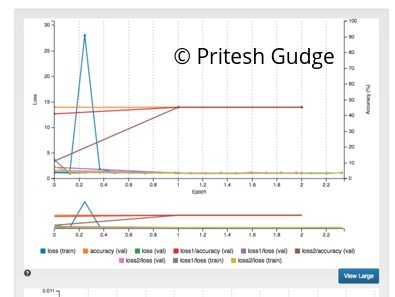
\includegraphics[width=\linewidth]{images/4_glenetadam_cropped_chart}
      \caption{Google Lenet Adam Optimization Bottless and Boxes: Training Progress Chart}
      \label{fig:boxes_adam_opt}
\end{figure}

In the next step the same Google LeNet network was used with standard SGD optimizer with 5 epochs and 0.01 learning rate at the start. 25\% of the dataset was used for validation. The test dataset was stored separately before training.
Once the model was found to be converging, the final model was set to train with an initial learning rate of 0.01 and 5 epochs of the network 22-layer Google LeNet.\cite{DBLP}. The test images were used to determine performance of the trained model. Speed of each individual classification run was also evaluated. Once trained the Google LeNet network model provides quick classification on GPU <10ms. 

\subsection{Food Classification}
6020 images were collected with approximately equal number of images for each of the classes:
\begin{itemize}
\item Banana
\item Guava
\item Other foods(Marshmallows)
\end {itemize}
Google Lenet\cite{DBLP} model was chosen for its effectiveness to classificiation and detection on ImageNet dataset as described above section \ref{googlelenet}. The hyperparameters: 10 epochs and a starting learning rate of 0.01 was chosen for training. 25\% of the dataset was used for validation. The test dataset was stored separately before training. The test images were used to determine performance of the trained model. Once trained the Google LeNet network model provides quick classification results on GPU and hence was chosen for this project. Eg. The model can be deployed on a TX2 processor and classification  results can be obtained real-time for the robotic platform in its operating state.

\begin{figure}[thpb]
      \centering
      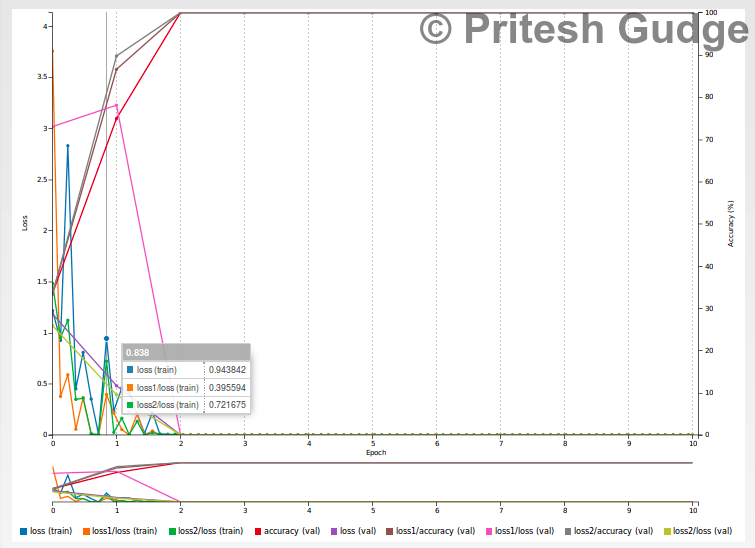
\includegraphics[width=\linewidth]{images/training_chart}
      \caption{Food Classification: Training Progress Chart}
      \label{fig:food_class1}
\end{figure}

%example for Bullet point list
%
%\begin{itemize}
%\item example
%\end {itemize}



%example for numbered list
%\begin{enumerate}
%\item example
%
%\end{enumerate}

\section{Data Acquisition}
\subsection{Bottles and Boxes}
The dataset was acquired by using a TX2 kit to capture images of boxes and bottles off a conveyor belt. The captured images were provided as standard in the \textit{Digits} workspace. Total of 10094 images were provide out of which 7570 images were used as training set and remaining 2524 were used as the validation set.


\subsection{Food Classification}
This dataset was collected by capturing images with a standard webcamera: \emph{Logitech 270} in diffused sunlight. The camera was connected to a Lenovo laptop (Figure \ref{fig:datacoll1}) using the USB port and images were captured by using a script\cite{capt_img_script}. The python language script used \emph{OpenCV} python library \textbf{cv2} to render and transform the images. 
2 varieties of guava and 1 variety of banana was taken for the fruits' classes of the dataset. These were the objects readily available while performing the data collection. Also, multi-colored marshmallows were available to describe the non-fruit(junk food) class.  6020 total images RGB images were captured, and resized to size 256x256 before storing into the appropriate classes Ref. Table \ref{table:fruit_table}.

\begin{figure}[thpb]
      \centering
      \includegraphics[width=\linewidth]{images/data_collection}
      \caption{Food Classification: Data Collection Setup}
      \label{fig:datacoll1}
\end{figure}


\begin{table}[h]
\caption{Fruit Images}
\label{table:fruit_table}
\begin{center}
\begin{tabular}{|c|c|}
\hline
      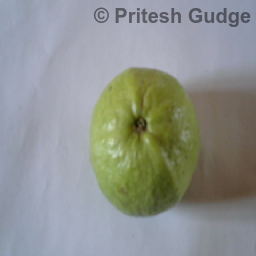
\includegraphics[width=1in]{images/Guava__395}
 &    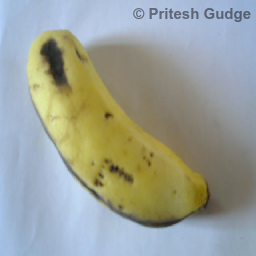
\includegraphics[width=1in]{images/Banana__1661}
       \\
%\hline
       Guava & Banana \\
\hline
\end{tabular}
\end{center}
\end{table}


%\begin{figure}[thpb]
%      \centering
%      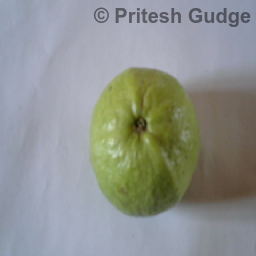
\includegraphics[width=1in]{images/Guava__395}
%      \caption{Guava Sample}
%      \label{fig:guava1}
%\end{figure}
%
%\begin{figure}[thpb]
%      \centering
%      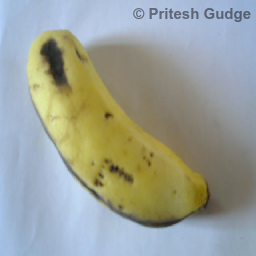
\includegraphics[width=1in]{images/Banana__1661}
%      \caption{Guava Sample}
%      \label{fig:guava1}
%\end{figure}
%

\section{Results}
\subsection{Bottles and Boxes}
The accuracy of Google Lenet Trained model with SGD optimizer was nearly 100\%. The learning stage loss and accuracy graphs are shown below Refer Figure: \ref{fig:boxes_learning} 

\begin{figure}[thpb]
      \centering
      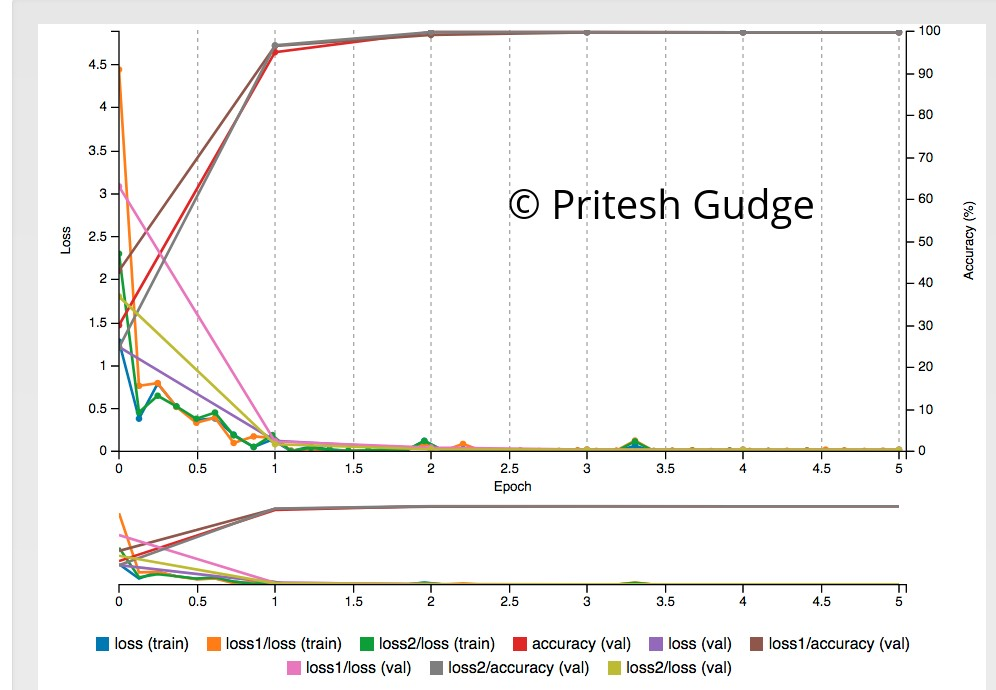
\includegraphics[width=\linewidth]{images/10_loss_accuracy}
      \caption{Boxes and Bottles: Learning Chart}
      \label{fig:boxes_learning}
\end{figure}

The results from the \emph{evaluate} command are shown in the figure \ref{fig:boxes_evaluate}. The average time for the evaluation runs is around 5 milliseconds which is within the provided constraint of it being below 10 milliseconds. The model accuracy is 75.40\% which is above the requirement minimum 75\% required from the implementation.


\begin{figure}[thpb]
      \centering
      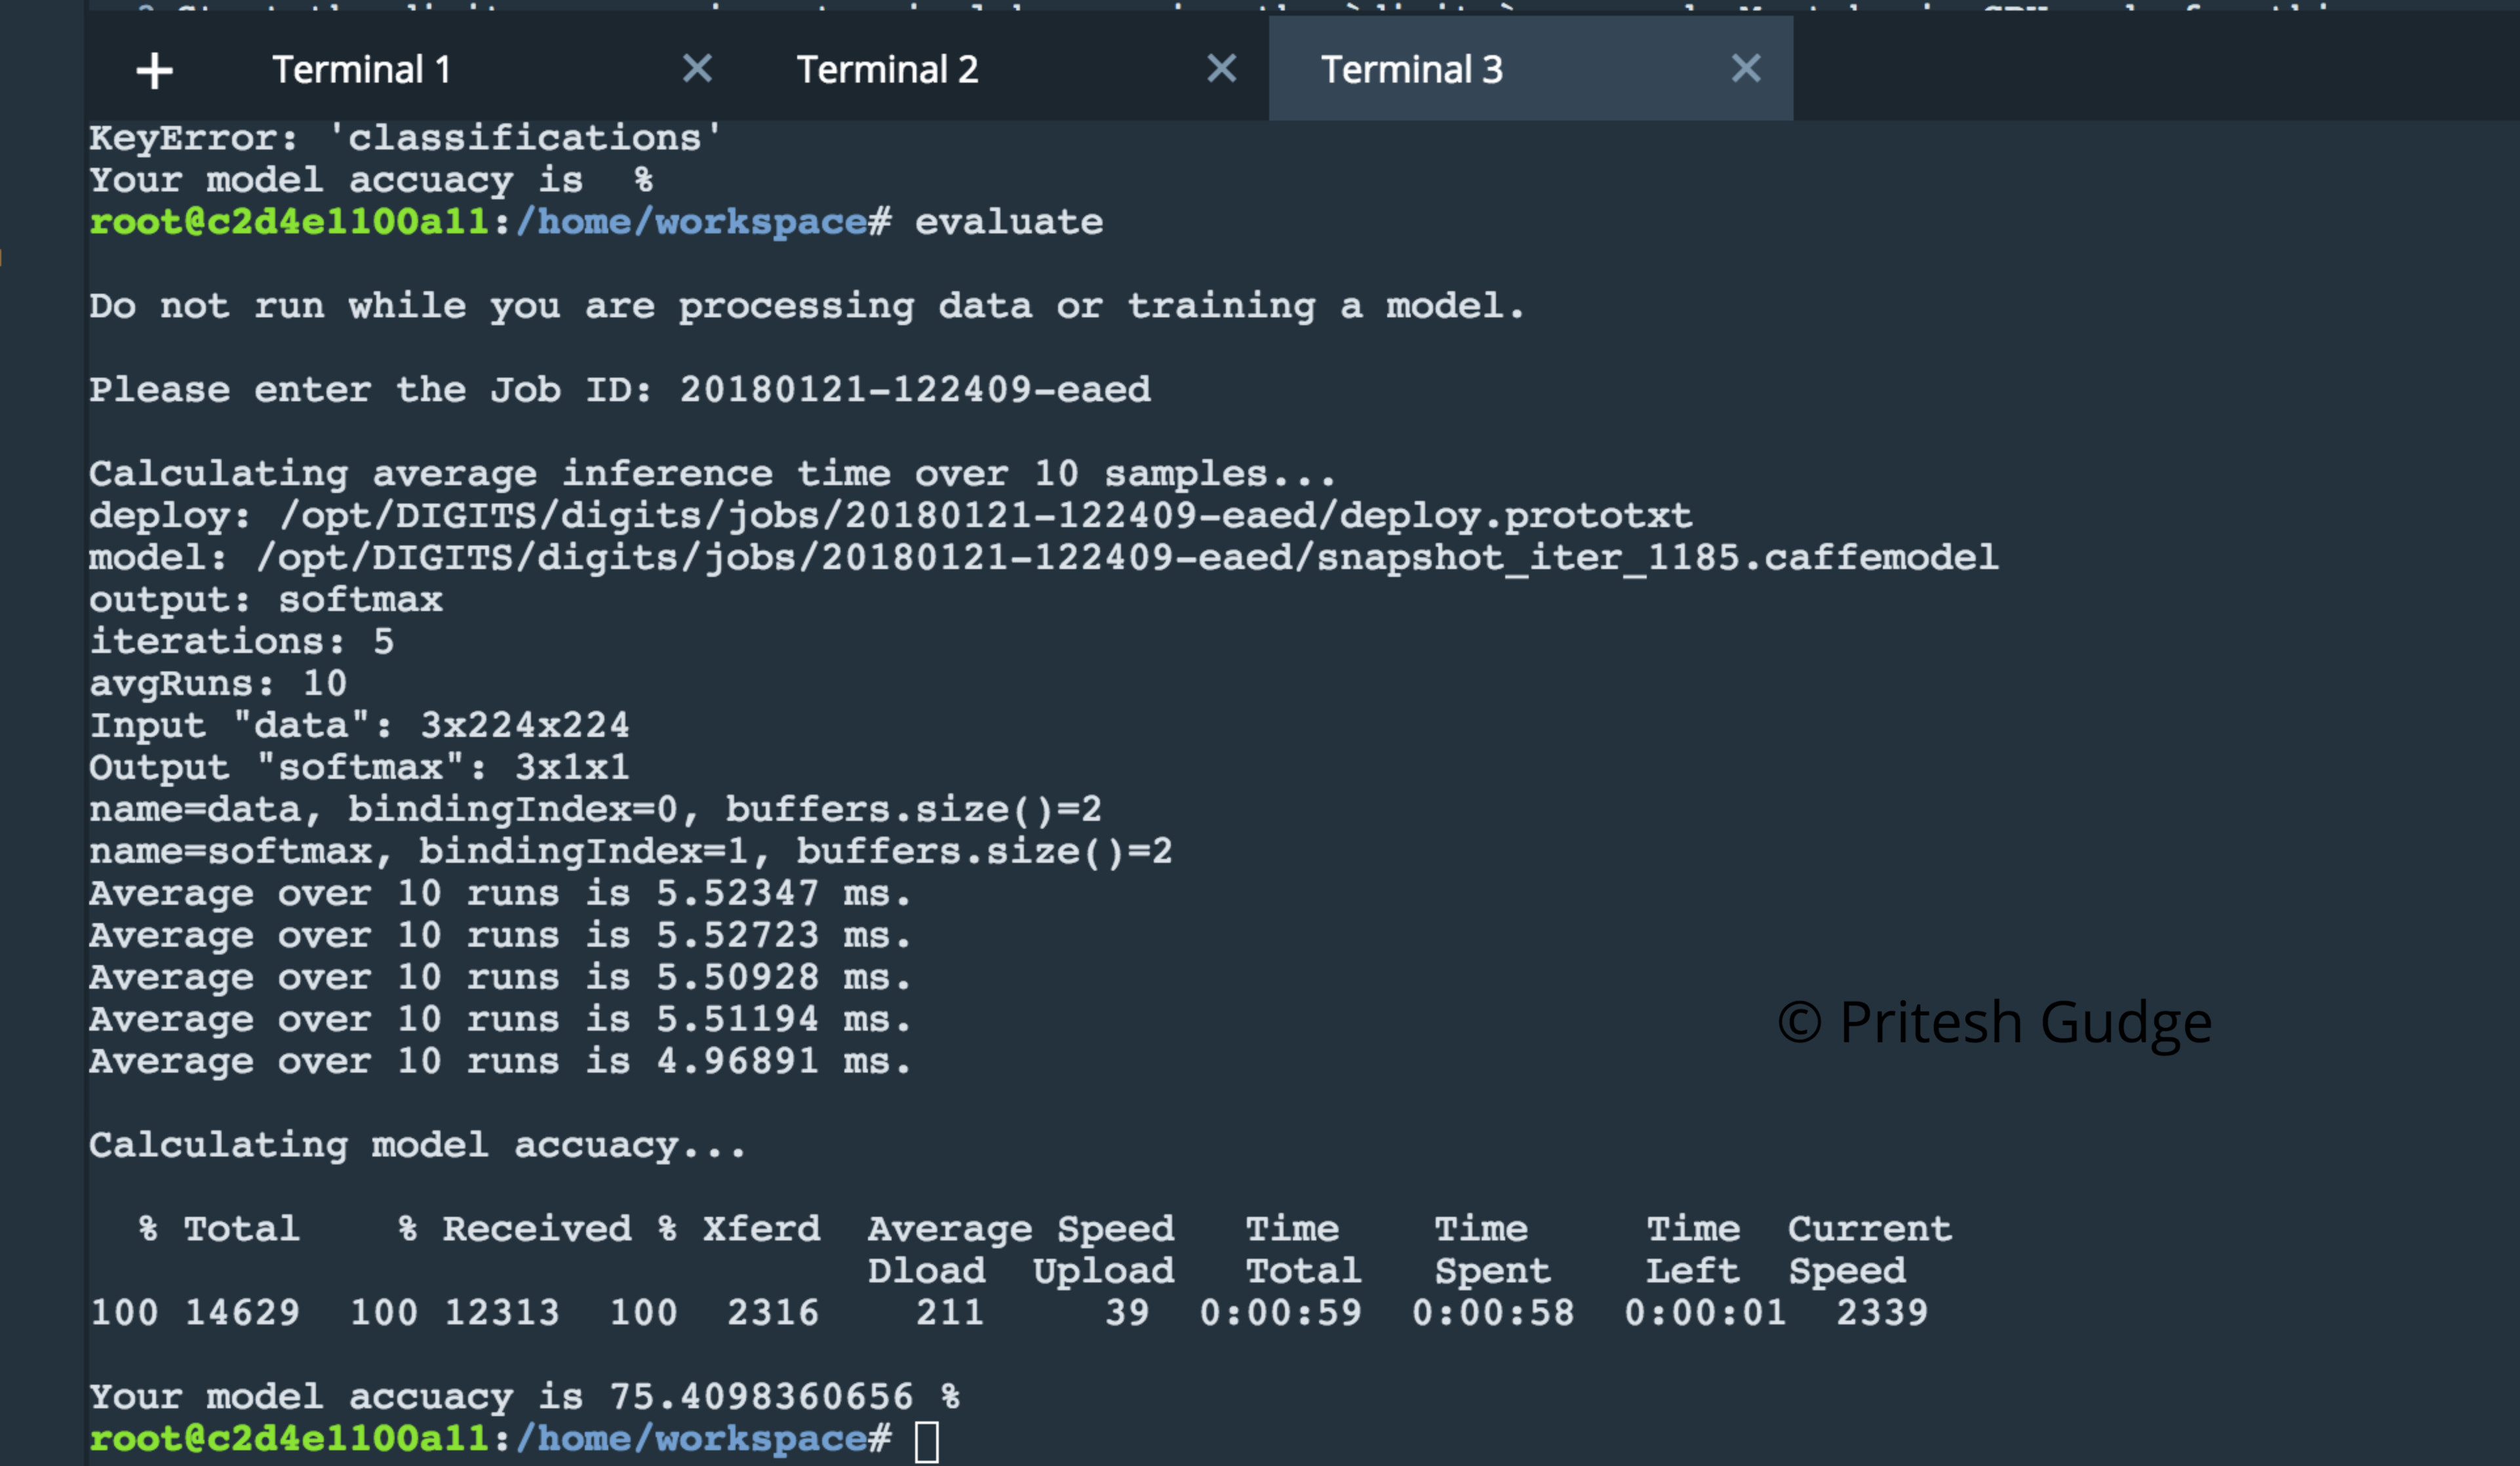
\includegraphics[width=\linewidth]{images/9_evaluate_screenshot2_watermarked}
      \caption{Boxes and Bottles: "evaluate" Command Result}
      \label{fig:boxes_evaluate}
\end{figure}

A sample classification run of one of the bottle images is shown below in figure \ref{fig:bottle_classify}. The accuracy for prediction is 99.87\%


\begin{figure}[thpb]
      \centering
      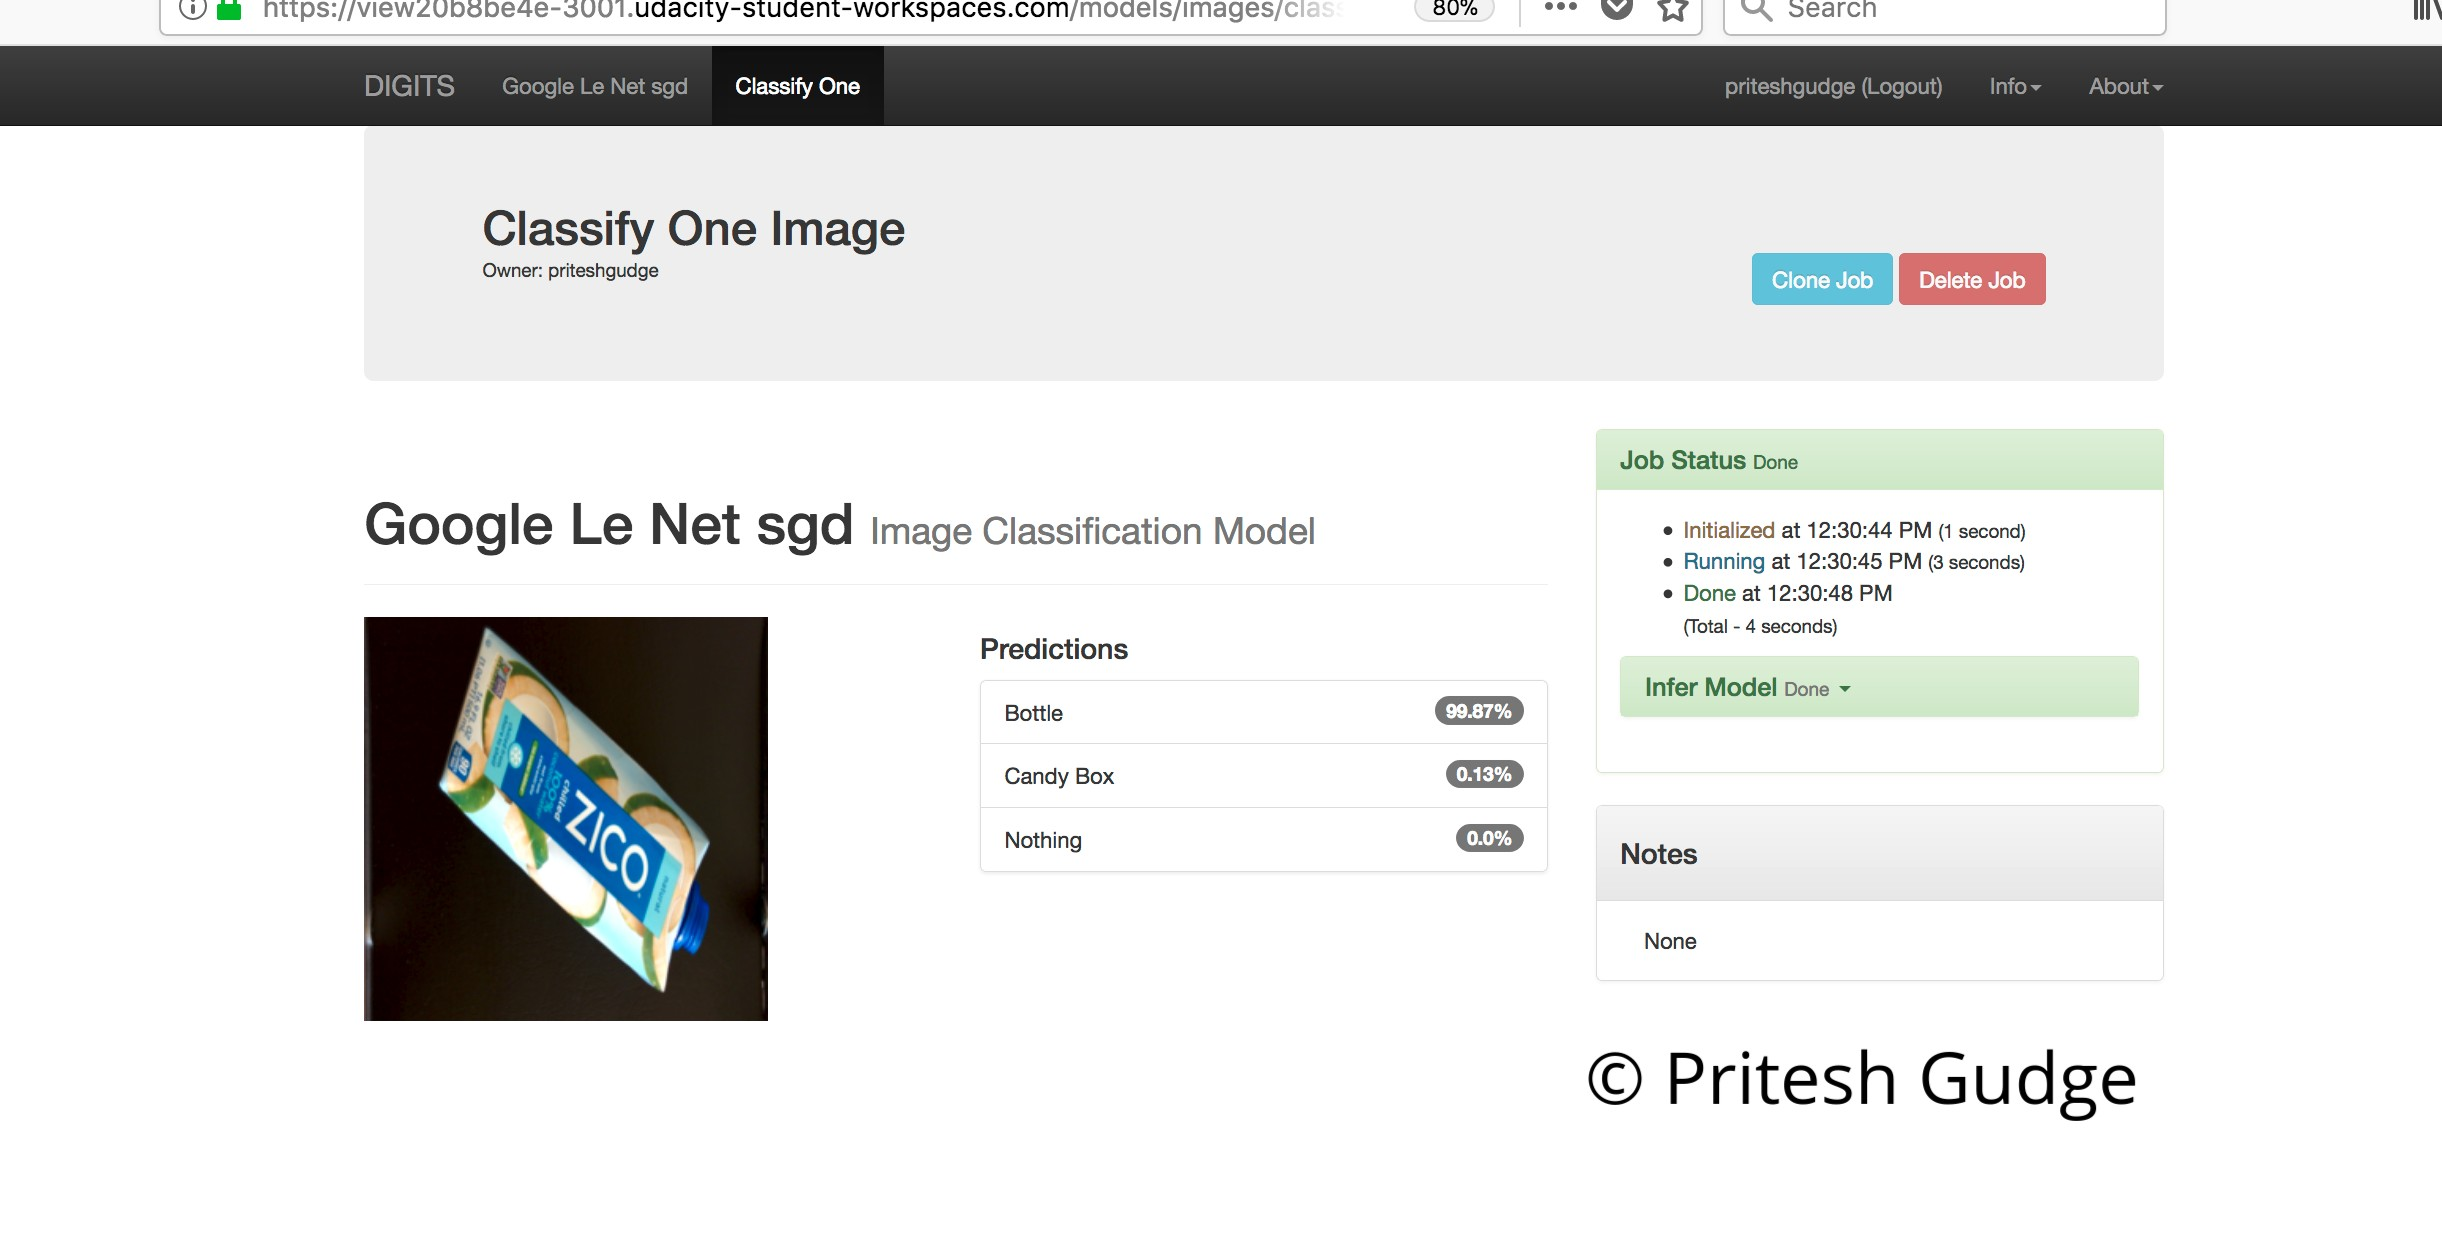
\includegraphics[width=\linewidth]{images/7_sgd_bottle}
      \caption{Boxes and Bottles: Sample Bottle Evaluation Result}
      \label{fig:bottle_classify}
\end{figure}

\subsection{Food Classification}
The classification performance from the food classification model for the included test images is satisfactory. The classification confidence is above 95\% for the images from the test dataset. The model appears to be overfitting according the the training chart Fig:\ref{fig:food_class1} and the resulting test image classification (Figures: \ref{fig:classify_many} \& \ref{fig:classify_guava}).

\begin{figure}[thpb]
      \centering
      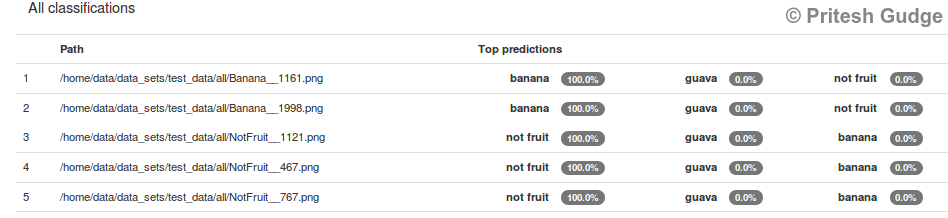
\includegraphics[width=\linewidth]{images/classify_many_2}
      \caption{Food Classification: Classify Many Result Show Overfitting}
      \label{fig:classify_many}
\end{figure}

\begin{figure}[thpb]
      \centering
      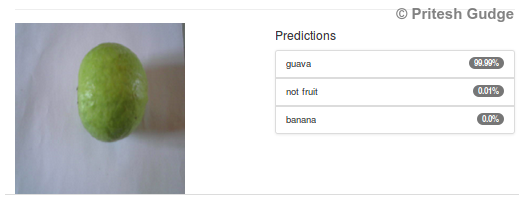
\includegraphics[width=\linewidth]{images/classify_guava_2}
      \caption{Classify Guava: Show Overfitting}
      \label{fig:classify_guava}
\end{figure}

%
%This is typically the hardest part of the report for many. You want to convey your results in an unbiased fashion. If you results are good, you can objectively note this. Similarly, you may do this if they are bad as well. You do not want to justify your results here with discussion; this is a topic for the next session. 
%Present the results of your robotics project model and the model you used for the supplied data with the appropriate accuracy and inference time
%For demonstrating your results, it is incredibly useful to have some charts, tables, and/or graphs for the reader to review. This makes ingesting the information quicker and easier.

\section{Discussion}
For the first part of the project, the classification confidence is above 75\% is satisfactory and meets the given requirements. The avearge evaluation time is also approximately 5 milliseconds. This meets the given requirement for evaluation time to be less than 10 milliseconds. The Google LeNet network is optimized for computation on GPU due to parallelization and high scale performance optimization \cite{DBLP}.

In the second part of the project, the model is overfitting the training data. Accuracy is near 99\% for the training model. Lower number of epochs, probably 3 or 4 epochs may help in preventing overfitting. More data needs to be collected to include different varieties of the fruits and junk food categories. The current model will be performant in a very narrow range of inputs. 

\section{Conclusion / Future work}
The first part of the project achieved the expected result. The evaluation performance was above 75\% and the evaluation time less than 10 milliseconds. This falls within the parameters of rubric requirements for the project. This model can be used in the future to build a sorting robot, which will sort objects into various bins. This can be useful for a robot which sorts trash for recycling. Extensive training with a huge variety of data will be required for this inference model to be viable for a commercial grade application.

For the second part, the work documented here achieves the objective of data collection, data conditioning, structuring and training of a model. The results from the evaluation for the limited test set are also satisfactory. This model can be used in a robotic application which will be mounted on a refrigerator/cupboard. When placing store bought items into the refrigerator/cupboard, the camera will capture the item and open the door only if it is healthy. Otherwise it will prompt the user to return the item. Another application can be junk food alert warning. An app can be used to record images of food consumed through the day. If junk food is consumed, the same will be flagged and an alert message will be sent to the user. 
For both the above applications to become commercially viable, the model will have to be trained on huge and varied dataset which captures all the commonly available processed and unprocessed foodstuffs.

\bibliography{bib}
\bibliographystyle{ieeetr}

\end{document}
